%% Source: https://github.com/tias/constraint-solving-course
%% Licensed under CC BY-NC-SA 4.0: https://creativecommons.org/licenses/by-nc-sa/4.0/
%% You may share and adapt this for non-commercial use,
%% with attribution and under the same license.

\documentclass{cons-beamer}

\usetikzlibrary{shadows,fit,tikzmark,backgrounds}
\usepackage{amsmath,amssymb}
\DeclareMathOperator*{\argmin}{argmin}
\DeclareMathOperator*{\argmax}{argmax}
\newcommand\blfootnote[1]{%
  \begingroup
  \renewcommand\thefootnote{}\footnote{
  \footnotesize #1
  \vspace*{1em}}%
  \addtocounter{footnote}{-1}%
  \endgroup
}
\definecolor{titles}{rgb}{0.65,0.1,0.1}
\newcommand{\gear}[5]{%
\foreach \i in {1,...,#1} {%
[rotate=(\i-1)*360/#1]  (0:#2)  arc (0:#4:#2) {[rounded corners=1.5pt]
         -- (#4+#5:#3)  arc (#4+#5:360/#1-#5:#3)} --  (360/#1:#2)
}%
(0,0) circle[radius=#2*0.5]
}
\newcommand{\paramsg}[2]{%
\node (#1) [#2] {
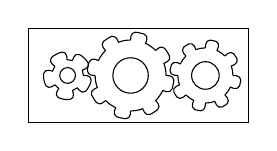
\begin{tikzpicture}
\draw[shift={(.2,.5)}] \gear{5}{.2}{.3}{20}{1};
\draw[shift={(1,.5)}] \gear{8}{.45}{.55}{20}{1};
\draw[shift={(1.95,.5)}] \gear{8}{.35}{.45}{20}{1};
\draw (-.3,-.1) -- (2.5,-.1) -- (2.5,1.1) -- (-.3,1.1) -- cycle;
\end{tikzpicture}
};
}

\begin{document}

\begin{frame}{L08: CP Search Strategies and Algorithm Configuration}
  \begin{center}
    ~ \\
    \includegraphics[height=42mm, trim=11px 8px 0 0, clip]{images/speedup} \\
    Prof. Tias Guns and Dr. Dimos Tsouros \\[0.5em]
    \includegraphics[width=2cm]{images/kuleuven_CMYK_logo.pdf}
  \end{center}
  
  {\footnotesize 
  Partly based on slides from Pierre Flener, Uppsala University and Lars Kotthoff, University of Wyoming.}
  % https://pierre-flener.github.io/courses/M4CO/lectures.html
\end{frame}

\begin{frame}{Goal of the lecture}
  Different solvers will behave differently for different problems...
  \vfill

  Typical CP problems are NP-hard, and we can not expect to solve all problems efficiently (unless P=NP).
  \vfill

  But many problems of practical interest:
  \begin{itemize}
    \item Can be practically solved
    \item Can be solved even faster with the right solving technology
    \item And even even faster with the right solver configuration:\\
          generic solvers include many \defined{design choices} and options to influence them.
  \end{itemize}
\end{frame}


\section{Varying propagation strengths}

\begin{frame}{CP solver structure}
  \centering
  \includegraphics[height=70mm]{images/cp_domain_store.png}
\end{frame}

\begin{frame}{Propagation strength}\label{propagator}
  \begin{definition}
    A \inference{propagator} for a predicate $\gamma$ deletes from the
    domains of the
    % decision
    variables of a~$\gamma$-constraint the values that cannot
    be in a solution to that constraint.
    \vfill 

    Not all impossible values need to be deleted:
    \begin{itemize}
      \item A \defined{domain-consistency (DC) propagator} deletes all
        impossible values from the domains.
      \item A \defined{bounds-consistency (BC) propagator} only deletes
        all impossible minimum and maximum values from the domains.
      \item A \defined{value-consistency (VC) propagator} is only awoken
        when at least one of its decision variables became fixed.
    \end{itemize}
  \end{definition}
  \vfill

  There exist other, unnamed consistencies for propagators. \vfill

  There is a trade-off between the time \& space complexity of a
  propagator and its achieved deletion of domain values.
\end{frame}

\begin{frame}
  \begin{example}[Linear equality constraints]
    Consider the linear constraint $3 * x + 4 * y = z$ \\
    with $\Domain{x} = \Set{0,1} =
    \Domain{y}$ and $\Domain{z} =
    \Set{0,\dots,10}$:
    \begin{itemize}
      \item A bounds-consistency propagator reduces
        $\Domain{z}$ to $\Set{0,\dots,7}$.
      \item A domain-consistency propagator reduces
        $\Domain{z}$ to $\Set{0,3,4,7}$.
    \end{itemize}
    \vfill

    Time complexity:
    \begin{itemize}
      \item A bounds-consistency propagator for a linear equality
        constraint can be implemented to run in $\Oh{n}$ time, where $n$
        is the number of decision variables in the constraint. 
      \item A domain-consistency propagator for a linear equality
        constraint can be implemented to run in $\Oh{n \cdot d^2}$ time,
        where $n$ is the number of decision variables in the constraint
        and $d$ is the sum of their domain sizes, hence in time
        pseudo-polynomial = exponential in the input magnitude.
    \end{itemize}
  \end{example}
\end{frame}

\begin{frame}{Controlling the CP Inference} 
  In the past, some solvers allowed users to set the propagation level for individual constraints (most notably the Gecode solver).
  \vfill

  Nowadays, solvers developers typically implement one (e.g. the strongest one) and run with it.
  \vfill

\end{frame}


\section{Search strategies}

\begin{frame}{Historic perspective}
  \textbf{CP as a depth-first search framework}
  \begin{itemize}    
    \item Historically, constraint programming solvers allow programming your own constraints as well as \defined{programmable search}:\\
      variable/value ordering and choices, e.g. which variables, what branching decision are created... also full access to the constraint and domain store.
  \end{itemize}

  \textbf{CP as generic satisfaction/optimisation solver}
  \begin{itemize}
    \item Since a number of years, the CP community has been advancing on 'the holy grail' of black box search strategies that work well in general, so users can especially focus on the modeling part.
    \item Solver-indendent modeling languages have taken one step further away from programmable search, allowing setting at most a variable/value ordering as a solver parameter.
  \end{itemize}
\end{frame}

\begin{frame}{Search Strategies}\label{searchCP}
  \search{Search Strategies:}
  \begin{itemize}
    \item On which decision variable to branch next?
    \item How to partition the domain of the chosen decision variable?
    \item Which search (depth-first, breadth-first, \dots) to use?
  \end{itemize}

  The search is usually depth-first search.
\end{frame}

\begin{frame}{Variable Selection Strategy}
  The variable selection strategy has an impact on the size of the
  search tree.
  \vfill

  \begin{example}[Impact of the variable selection strategy]
    Consider $x \in \Set{1,2}$, $y \in \Set{1,2,3,4}$, $z \in \Set{1,\dots,6}$, \\
    branching on all domain values, but no constraints: \vfill
    \begin{itemize}
      \item If selecting the decision variables in the order
        $x, y, z$, then the CP search tree has 
        $1 + 2 + 2 \cdot 4 + 2 \cdot 4 \cdot 6 = 59$
        nodes and $2 \cdot 4 \cdot 6 = 48$ leaves.
        \vfill

      \item If selecting the decision variables in the order
        $z, y, x$, then the CP search tree has
        $1 + 6 + 6 \cdot 4 + 6 \cdot 4 \cdot 2 = 79$
        nodes and also $6 \cdot 4 \cdot 2 = 48$ leaves.
    \end{itemize}
  \end{example}
\end{frame}

\begin{frame}\label{var}
  \begin{definition}[First-Fail Principle]
    To succeed, first try where you are most likely to fail. 
    In practice:
    \begin{itemize}
      \item Select a decision variable with the smallest current domain.
      \item Select a decision variable involved in the largest number of constraints.
      \item Select a decision variable recently causing the most backtracks.
    \end{itemize}
  \end{definition}
  \vfill

  \begin{example}[Impact of the variable selection strategy]
    Finding the first solution to $250$-queens with CPMpy-Choco
    (CP):
    \begin{center}
      %% on Tias' intel laptop, Nov 2024
      \begin{tabular}{lrr}
        search & seconds \\
        \midrule
        default & 0.17 \\
        smallest-domain, lb value & 0.19 \\
        conflict-history search & 0.22 \\
        activity-based search & 0.23 \\
        domain size over weighted degree & $>30$ \\
        input order, lb value & $>30$ \\
        %failure rate-based search & >30
      \end{tabular}
    \end{center}
  \end{example}
\end{frame}

\begin{frame}{Domain Partitioning Strategy}
  (including value orderings)\vfill

  \begin{example}[Impact of the domain partitioning strategy]
    Consider $x \in \Set{1,2}$, $y \in \Set{1,2,3,4}$, $z \in \Set{1,\dots,6}$, \\
    domain consistency for $x * y = z$, $x \neq y$, $x \neq z$, and $y \neq z$, \\
    smallest-domain variable selection, and depth-first search:

    \begin{itemize}
      \item If the domain is split into singletons by increasing order, \\
        then $6$ CP nodes are explored before finding the (unique) solution.

      \item If the domain is split into singletons by decreasing order, \
        then only $2$ CP nodes (the root and a leaf) are explored \\
        before finding the (unique) solution, without backtracking.
    \end{itemize}
  \end{example}
\end{frame}

\begin{frame}\label{varval}
  \begin{definition}[Best-First Principle]
    First try a domain part that is most likely, if not guaranteed, to
    have values that lead to solutions.
  \end{definition} \vfill%

  This may be like how one would make the greedy choice in a greedy
    algorithm for the problem at hand, considering its objective
    function.
    
  \begin{example}[Impact of the domain partitioning strategy]
    %(Continued from slide~\ref{var}) \\ 
    Finding the first solution to $750$-queens with CPMpy-Choco
    \begin{center}
      %% on Tias' intel laptop, Nov 2024
      \begin{tabular}{lrr}
        search & seconds \\
        \midrule
        smallest-domain, lb value & 3.35 \\
        smallest-domain, ub value & 2.88 \\
      \end{tabular}
    \end{center}
  \end{example}
\end{frame}


\section{Other design choices}

\begin{frame}{Other search strategies}
  \begin{description}
    \item[warmstarting] if a previous solution is known \\
    or a \textit{solution hint}: what value to try first for specific variables (very useful in repeated solving)

    \item[heuristics/local search] to quickly find a feasible solution\\
        provides an upper bound (for minimisation problems), good user experience

    \item[probing\hfill] try assigning a variable to a value and propagate it (no search), derives failing values, or hidden consequences (e.g. if comparing propagation effect of assigning a Boolean variable to True and to False)
    
    \item[restarts during search] for clause learning solvers, backjump to the root node.\\
    Can be very effective (because variable activity was updated during previous search, so most active variables are now at 'top' of the tree)
  \end{description}
\end{frame}

\begin{frame}{Other solver configuration options}
    These are often very solver-specific!!
    \vspace{1em}

    \textbf{OrTools CP-SAT}: %\footnote{\url{https://github.com/google/or-tools/blob/stable/ortools/sat/sat_parameters.proto}}:} 
    \begin{itemize}
      \item "cp\_model\_probing\_level": how much effort on probing
      \item "search\_branching": search strategy (automatic, fixed, hint, LP-based, ...)
      %\item "linearization\_level": which constraints to add to LP relaxation
      \item "symmetry\_level": symmetry detection and breaking before/during search
      \item "use\_phase\_saving": value selection = last value the variable was assigned to
    \end{itemize}

    \textbf{Choco}: %\footnote{\url{https://github.com/chocoteam/pychoco/blob/master/pychoco/backend.i}}:
    In Python API only some search strategies are exposed. Java API: programmable search and tons of options!

    \textbf{Gurobi} categories: %\footnote{\url{https://docs.gurobi.com/projects/optimizer/en/current/concepts/parameters/groups.html#secparametergroups}} categories:
    \begin{itemize}
      \item Tolerance parameters which control solution quality requirements
      \item Algorithmic control parameters for Presolve, Simplex, Barrier, Scaling, MIP and MIP Cuts%, and Numerics;
    \end{itemize}
\end{frame}


\section{Algorithm Selection and Configuration}

\begin{frame}{Algorithm Selection and Configuration}

  Which solver to use? Which choices to make?
  \vspace{1em}

  \begin{description}
    \item[Algorithm Selection] choose the best \emph{algorithm} for solving a
    problem
    \item[Algorithm Configuration] choose the best \emph{parameter configuration}
  \end{description}
  \vspace{1em}

  Large performance improvements possible, without changing the model!
  \blfootnote{Based on slides from Lars Kotthoff, Univ of Wyoming}
\end{frame}

\begin{frame}{Performance Improvements example}
  \begin{center}
    \includegraphics[height=.68\textheight]{images/speedup}
  \end{center}
  \blfootnote{%
  Hutter, Frank, Domagoj Babic, Holger H. Hoos, and Alan J. Hu. ``Boosting
  Verification by Automatic Tuning of Decision Procedures.'' FMCAD 07.
  }
\end{frame}

\begin{frame}{Algorithm Selection}
  \begin{center}
    Given a problem, choose the best algorithm to solve it.
  \end{center}
  

	``algorithm'' used in a very loose sense
	\begin{itemize}
		\item constraint solvers
		\item search strategies
		\item modelling choices
		\item different types of consistency
		\item \ldots
	\end{itemize}

  As long as a finite (typically small) set of "algorithms" is available: the \textit{portfolio}.

  \blfootnote{Rice, John R. ``The Algorithm Selection Problem.'' Advances in Computers 15 (1976): 65–118.}
\end{frame}

\begin{frame}{Building an Algorithm Selection System}

Most often 'instance specific' algorithm configuration:

\begin{itemize}
	\item For an unseen instance: which algorithm (from the finite set) should I run?
	\item Instance-specific: allowed to analyse the instance and decide based on \textit{features} that you can derive from it
	\begin{itemize}
		\item nr of variables, constraints
		\item types of constraints used
		\item constraint network (e.g. GNNs)
		\item probing (run an algorithm for short time, collect statistics)
	\end{itemize}
	\item Most often Machine Learning is used to build a \textbf{performance model},\\ and predict which algorithm to use.
\end{itemize}
\end{frame}

\begin{frame}{Types of Performance Models}
\begin{center}
\resizebox{!}{.8\textheight}{%
\tikzset{>=latex}
\begin{tikzpicture}[node distance=1em,inner sep=.5em,n/.style={drop shadow,fill=white,rounded corners}
]

\node (pm2c) [n,align=center,draw] {Regression Models\\
\begin{tikzpicture}[scale=0.3]
\draw (0,1) .. controls (1,1) .. (4,0) node [right]{A1};
\draw (0,0) .. controls (1,0) .. (4,4) node [right]{A2};
\draw (0,2) .. controls (2,3) .. (4,2) node [right]{A3};
\end{tikzpicture}
};

\node (pm2cr) [align=left,right=3em of pm2c] {A1: 1.2\\\textbf{A2: 4.5}\\A3: 3.9};

\node (pm1c) [n,align=center,above=of pm2c,draw] {Classification Model\\[1em]
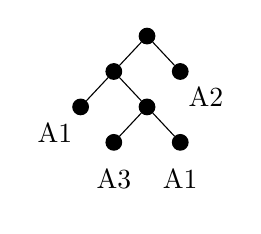
\begin{tikzpicture}[scale=0.3,sibling distance=8em,every node/.style={circle,fill=black,inner sep=.2em}]
\node (pm1) [draw] {}
child{ node [draw] {}
        child{ node [draw,label={below left:A1}] {} }
        child{ node [draw] {}
                        child{ node [draw,label={below:A3}] {}}
                        child{ node [draw,label={below:A1}] {}}
        }
}
child{ node [draw,label={below right:A2}] {} }
;
\end{tikzpicture}
};

\node (pm1cr) [align=left,right=3em of pm1c] {\textbf{A1}};

\node (pm3c) [n,align=center,below=of pm2c,draw] {Pairwise Classification Models\\[1em]
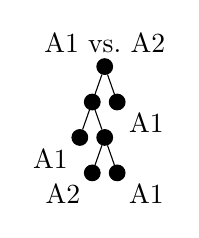
\begin{tikzpicture}[scale=0.3,every label/.append style={shape=rectangle},sibling distance=3em,every node/.style={circle,fill=black,inner sep=.2em}]
\node [draw,label={above:A1 vs.\ A2}] {}
child{ node [draw] {}
        child{ node [draw,label={below left:A1}] {} }
        child{ node [draw] {}
                        child{ node [draw,label={below left:A2}] {}}
                        child{ node [draw,label={below right:A1}] {}}
        }
}
child{ node [draw,label={below right:A1}] {} }
;
\end{tikzpicture}
\hspace{1em}
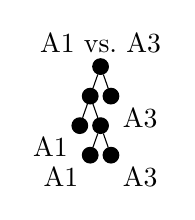
\begin{tikzpicture}[scale=0.25,every label/.append style={shape=rectangle},sibling distance=3em,every node/.style={circle,fill=black,inner sep=.2em}]
\node [draw,label={above:A1 vs.\ A3}] {}
child{ node [draw] {}
        child{ node [draw,label={below left:A1}] {} }
        child{ node [draw] {}
                        child{ node [draw,label={below left:A1}] {}}
                        child{ node [draw,label={below right:A3}] {}}
        }
}
child{ node [draw,label={below right:A3}] {} }
;
\end{tikzpicture}
\hspace{1em}
\raisebox{3.7em}{\ldots}
};

\node (pm3cr) [align=left,right=1em of pm3c] {A1: 1 vote\\A2: 0 votes\\\textbf{A3: 2 votes}};

\node (pm4c) [n,align=center,below=of pm3c,draw] {Pairwise Regression Models\\[1em]
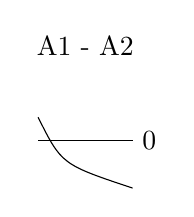
\begin{tikzpicture}[scale=0.3]
\draw (2,6) node {A1 - A2};
\draw (0,3) .. controls (1,1) .. (4,0);
\draw (0,2) -- (4,2) node [right] {0};
\end{tikzpicture}
\hspace{1em}
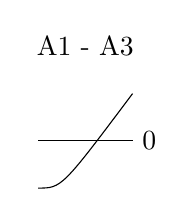
\begin{tikzpicture}[scale=0.3]
\draw (2,6) node {A1 - A3};
\draw (0,0) .. controls (1,0) .. (4,4);
\draw (0,2) -- (4,2) node [right] {0};
\end{tikzpicture}
\hspace{1em}
\raisebox{2em}{\ldots}
};

\node (pm4cr) [align=left,right=1em of pm4c] {A1: -1.3\\A2: 0.4\\\textbf{A3: 1.7}};

\node (pmc) [fit={(pm1c) (pm1cr) (pm2c) (pm2cr) (pm3c) (pm3cr) (pm4c) (pm4cr)},draw,dashed] {};

\node (it) [align=center,left=3em of pmc] {Instance 1\\Instance 2\\Instance 3\\ $\vdots$};

\node (ps) [align=center,right=3em of pmc] {Instance 1: Algorithm 2\\Instance 2:
Algorithm 1\\Instance 3: Algorithm 3\\ $\vdots$};

\path [->] (it) edge (pmc);
\path [->] (pmc) edge (ps);
\path [->] (pm1c) edge (pm1cr);
\path [->] (pm2c) edge (pm2cr);
\path [->] (pm3c) edge (pm3cr);
\end{tikzpicture}}
\end{center}
\end{frame}

\begin{frame}{Algorithm Configuration = Automated Parameter Tuning}
  \begin{center}
  \[
    \tikzmarknode{alg}{\lambda^*} \in
    \tikzmarknode{min}{\argmax_{\lambda\in\Lambda}}\,
    \tikzmarknode{ge}{p}
    \tikzmarknode{model}{\left(\mathcal{A}_{\lambda}, \mathcal{D}\right)}
  \]
  \begin{tikzpicture}[overlay,remember picture,>=stealth,nodes={align=left,inner ysep=1pt},<-]
    \path (alg.south) ++ (-5em,-1.5em) node[anchor=north,color=titles] (alglabel) {Find a parameter setting};
    \draw [color=titles] ([yshift=-1ex] alg.south) |- ([xshift=-1em] alglabel.north);

    \path (min.south) ++ (0,-3.5em) node[anchor=north,color=titles] (minlabel) {that maximizes};
    \draw [color=titles] ([yshift=-1ex] min.south) |- (minlabel.north);

    \path (ge.north) ++ (0,+1.5em) node[anchor=south,color=titles] (gelabel) {the performance};
    \draw [color=titles] ([yshift=+1ex] ge.north) |- (gelabel.south);

    \path (model.south) ++ (3em,-1.5em) node[anchor=north,color=titles] (modellabel)
        {of the algorithm on\\the input data.};
    \draw [color=titles] ([yshift=-1ex] model.south) |- (modellabel.north);
  \end{tikzpicture}
  \end{center}
\end{frame}

\begin{frame}{Parameters?}
  \begin{itemize}
    \item anything you can change that makes sense to change
    \item typically multiple parameters with many values (possible continuous): a \textbf{large} (possibly infinite) set
    \item e.g.\ search heuristic, variable ordering, type of global constraint decompositions, presolve settings, different thresholds, ...
    \item Example: CPLEX MIP solver, 76 parameters; Spear SAT solver, 26 parameters
  \end{itemize}
  \vspace{1em}

  Typically for a \textit{set} of related instances (e.g. nurse rostering problems that the hospital solves every day)
\end{frame}

\begin{frame}{Algorithm Configuration}
  \includegraphics[width=0.9\textwidth]{images/ac}

  \blfootnote{Frank Hutter and Marius Lindauer, ``Algorithm Configuration: A Hands on
  Tutorial'', AAAI 2016}
\end{frame}

\begin{frame}{Grid and Random Search}
  \includegraphics[height=.7\textheight]{images/grid-random}
  \blfootnote{Bergstra, James, and Yoshua Bengio. ``Random Search for
  Hyper-Parameter Optimization.'' J. Mach. Learn. Res. 13, no. 1 (February 2012):
  281–305.}
\end{frame}

\begin{frame}{Model-Based Optimization}
  \begin{itemize}
    \item evaluate small number of initial (random) configurations
    \item use (probabilistic) Machine Learning to train a surrogate model of parameter-performance surface based on this
    \item use \textit{acquisition function} to decide most promising configuration to try next
    \item repeat, stop when resources exhausted or desired solution quality achieved
  \end{itemize}
  \vspace{1em}

  Allows targeted exploration of a limited number of promising configurations (time budget).
\end{frame}

\begin{frame}{Model-Based Optimization}
\begin{center}
\scalebox{0.6}{%
\tikzset{>=latex}
\begin{tikzpicture}[node distance=1em,inner sep=.5em,n/.style={drop shadow,fill=white,rounded corners}]

\node (sc) [n,align=center,draw] {\textbf{Surrogate Model}\\[1em]
\begin{tikzpicture}[scale=0.3]
\draw plot coordinates {(0,1) (1,1) (2,0) (3,1.5) (4,2) (5,0) (6,3) (7,2.5) (8,2)};
\end{tikzpicture}
};

\node (pc) [n,align=left,below right=-.7em and 7em of sc,draw] {\textbf{Parameter Configuration}\\[.5em]
Parameter 1: 7.5\\
Parameter 2: 0\\
Parameter 3: -3};

\paramsg{ge}{below=3em of sc};
\node (up) [align=center,below=0em of ge] {\textbf{Expensive-to-Evaluate Process}\\ \textbf{to be Optimized}};

\node (ac) [align=left] {};

\begin{pgfonlayer}{background}
\node (conf) [n,inner sep=1em,fit={(ac) (sc) (pc) (up) (ge)},draw] {};
\node (upc) [n,fit={(up) (ge)},draw] {};
\end{pgfonlayer}

\node (psc) [n,align=left,above right=3em of conf.east,draw] {\textbf{Parameter Space}\\[.5em]
Parameter 1: $[5..100]$\\
Parameter 2: $[0..10]$\\
Parameter 3: $[-10..10]$};

\node (m) [align=left,below=3em of conf] {\textbf{Parameter 1: 5}\\\textbf{Parameter 2: 2.1}\\\textbf{Parameter 3: -0.3}};

\path [->] (psc) edge (conf);

\path [->,thick,bend left=15] (pc) edge node [below] {evaluate} ([xshift=-5pt]ge.east);
\path [->,thick,bend left=75] ([xshift=5pt]ge.west) edge node [right] {observe} (sc.west);
\path [->,thick,bend left=20] (sc) edge node [above right] {propose} (pc);

\path [->] (conf) edge (m);
\end{tikzpicture}}
\end{center}
\end{frame}

% Generating next 3 slides automatically
\foreach \i in {2,3,4}{
\begin{frame}{Sequential Model-Based Optimization (SMBO) Example}
  \begin{center}
    \includegraphics[page=1,height=.63\textheight]{images/mbo-\i}  % images/mbo-2 images/mbo-3 images/mbo-4
  \end{center}

  \blfootnote{Bischl, Bernd, Jakob Richter, Jakob Bossek, Daniel Horn, Janek Thomas,
  and Michel Lang. ``MlrMBO: A Modular Framework for Model-Based
  Optimization of Expensive Black-Box Functions,''}
\end{frame}
}

\begin{frame}{Time Budget}
	How much time/how many function evaluations?
	\begin{itemize}
		\item too much $\to$ wasted resources
		\item too little $\to$ suboptimal result
		\item use statistical tests?
		\item evaluate on parts of the instance set
		\item for runtime: adaptive capping = solver timeout with current best runtime.
	\end{itemize}
  \vspace{1em}
    
  Need to evaluate on an unseen test-set to avoid 'over-tuning'.
\end{frame}


\begin{frame}{Summary}
  \begin{description}
    \item[Algorithm Selection] choose the best \emph{algorithm} for solving a problem
    \item[Algorithm Configuration] choose the best \emph{parameter configuration}
      for solving a problem with an algorithm
  \end{description}
  \vspace{1em}

  \begin{itemize}
    \item mature research areas
    \item can combine configuration and selection
    \item effective tools are available (e.g. HyperOpt, does SMBO (without adaptive capping...))
  \end{itemize}
\end{frame}

\end{document}
